\documentclass[11pt,a4paper]{article}
\usepackage[T1]{fontenc}
\usepackage[utf8]{inputenc}
\usepackage{newtxtext,newtxmath}
\usepackage{microtype}
\setlength{\emergencystretch}{1em}
\usepackage[margin=23mm,headheight=14pt]{geometry}
\usepackage{booktabs,tabularx,array,caption,float}
\usepackage{amsmath,tikz}
\usetikzlibrary{arrows.meta}
\usepackage{xcolor,fancyhdr,lastpage}
\usepackage[hidelinks]{hyperref}
\definecolor{accent}{HTML}{254C58}
\hypersetup{pdftitle={Q1.1 and Q1.2 -- NKT 33 kV Cable},pdfauthor={Tiebert Lefebure}}
\pagestyle{fancy}\fancyhf{}
\fancyhead[L]{\small Finite Elements for Electromagnetic Fields}
\fancyhead[R]{\small NKT 33 kV XLPE-AL}
\fancyfoot[L]{\small Cable selection and environment}
\fancyfoot[R]{\small \thepage\,/\,\pageref{LastPage}}
\renewcommand{\headrulewidth}{0.3pt}
\setlength{\parindent}{0pt}\setlength{\parskip}{6pt}
\setlength{\tabcolsep}{7pt}\renewcommand{\arraystretch}{1.19}
\captionsetup{font=small,labelfont=bf,skip=7pt}
\newcolumntype{Y}{>{\raggedright\arraybackslash}X}
\newcommand{\subhead}[1]{\par\medskip{\large\bfseries #1}\par\smallskip}
\newcommand{\source}[2]{\href{#1}{\textit{#2}}}
\begin{document}
{\LARGE\bfseries Cable selection and material data}\par
{\large Q1.1 --- Cable description}\par\medskip

The selected cable is the \textbf{NKT 33 kV single-core XLPE-AL,
\(1\times240+50~\mathrm{mm^2}\)}. Three identical cables form the three-phase
system. Each has a \(240~\mathrm{mm^2}\) aluminium conductor and a
\(50~\mathrm{mm^2}\) copper wire screen [1].

From the centre outward, the construction comprises a circular solid aluminium
conductor, a semiconducting conductor screen, XLPE insulation, a semiconducting
insulation screen, copper wires with a counter-wound copper tape, and a black
polyethylene (PE) outer sheath.

\begin{table}[H]
\centering
\caption{Geometrical data of the selected NKT cable [1].}\label{tab:geometry}
\begin{tabularx}{\linewidth}{@{}Y r@{}}
\toprule
Parameter & Dimension \([\mathrm{mm}]\)\\
\midrule
Aluminium conductor diameter & 17.0\\
Inner semiconductor thickness & Not specified\\
XLPE insulation thickness & 8.0\\
Outer semiconductor thickness & Not specified\\
Diameter over insulation & 34.6\\
Diameter over copper wire screen & 40.3\\
PE outer sheath thickness & 2.3\\
Overall cable diameter, nominal & 45.5\\
Overall cable diameter, maximum & 49.5\\
\bottomrule
\end{tabularx}
\end{table}
{\small Thicknesses are radial. The copper screen is a wire layer with a
\(50~\mathrm{mm^2}\) metallic area; the complete screen region must not be
represented as solid copper. Unspecified layer dimensions require explicit
geometry assumptions.}

\begin{table}[H]
\centering
\caption{Electromagnetic and thermal properties adopted for the initial model.}
\label{tab:materials}\small
\begin{tabularx}{\linewidth}{@{}Y c c c c l@{}}
\toprule
Material & \(\varepsilon_r\) & \(\mu_r\) &
\(\sigma~[\mathrm{S/m}]\) & \(\kappa~[\mathrm{W/(m\,K)}]\) & Sources\\
\midrule
Aluminium & \(1^\ast\) & \(1^\dagger\) & \(3.65\times10^7\) & 237 & [2]\\
Copper & \(1^\ast\) & \(1^\dagger\) & \(5.95\times10^7\) & 402 & [2]\\
Semiconducting PE & 2.25 & \(1^\dagger\) & \(2\times10^{-3}\) & 0.286 & [2]\\
XLPE & 2.5 & \(1^\dagger\) & \(10^{-18}\) & 0.286 & [3,4]\\
PE sheath & 2.25 & \(1^\dagger\) & \(10^{-18}\) & 0.46 & [5]\\
Soil & 10 & \(1^\dagger\) & \(10^{-2}\) & 0.833 & [1,A]\\
\bottomrule
\end{tabularx}
\end{table}
{\small
\(\varepsilon_r\): relative permittivity; \(\mu_r\): relative permeability;
\(\sigma\): electrical conductivity; \(\kappa\): thermal conductivity.
Metal conductivities refer to approximately room temperature.

For XLPE, \(\varepsilon_r\) and \(\kappa\) follow [3], and \(\sigma\) follows [4].
For soil, \(\varepsilon_r\) and \(\sigma\) follow Appendix C [A], while
\(\kappa=1/1.2\) follows the NKT rating condition [1].
All \(\mu_r\) values use the nonmagnetic approximation in [A].
These are cited modelling assumptions, not NKT-certified compound data.}

\newpage
{\large\bfseries Q1.1 --- Rating, assumptions and sources}\par\medskip

The \textbf{continuous ampacity is \(415~\mathrm{A~RMS}\) per phase} for the
conditions in Table~\ref{tab:rating}. This is the datasheet's ground-installation,
both-ends-bonded, touching-trefoil row in the \(240~\mathrm{mm^2}\) column [1].
The model frequency is \(50~\mathrm{Hz}\).

\begin{table}[H]
\centering
\caption{Rated quantities and the corresponding laying conditions [1].}
\label{tab:rating}
\begin{tabularx}{\linewidth}{@{}l Y@{}}
\toprule
Quantity & Selected value\\
\midrule
Rated voltage & \(33~\mathrm{kV~RMS}\), between phases\\
Continuous ampacity & \(415~\mathrm{A~RMS}\), per phase\\
Installation & Direct burial in the ground\\
Cable arrangement & Three cables touching in trefoil, \(S=D\)\\
Copper-screen bonding & Screens bonded at both ends\\
Burial depth & \(1.0~\mathrm{m}\)\\
Undisturbed ground temperature & \(15~^\circ\mathrm{C}\)\\
Soil thermal resistivity & \(1.2~\mathrm{K\,m/W}\)\\
Maximum conductor temperature & \(90~^\circ\mathrm{C}\), continuous operation\\
\bottomrule
\end{tabularx}
\end{table}

\subhead{Material assumptions}
\(\boldsymbol{\ast}\) \textbf{Metal permittivity.}
The value \(\varepsilon_r=1\) follows the convention in [2] and [A].
Conduction dominates displacement current in aluminium and copper at \(50~\mathrm{Hz}\),
so this placeholder has negligible influence.

\(\boldsymbol{\dagger}\) \textbf{Magnetic properties.}
All materials are treated as nonmagnetic, \(\mu_r=1\), consistently with
Appendix C [A]. This cable contains no steel armour.

\textbf{Polymers and temperature.}
Semiconducting PE represents both semiconducting layers [2]. The XLPE thermal
conductivity follows the cable-rating reference [3]. These are initial constant
properties; temperature-dependent metal conductivity is needed in the later coupled model.

\subhead{References}
\begingroup\small\setlength{\parskip}{6pt}
[1] NKT, \textit{33 kV single core cable XLPE-AL Halogen free},
printed pp.~19--20, \(240~\mathrm{mm^2}\) column.
\source{https://nkt.widen.net/content/d8gut55fhb/pdf/33kV_1-core_XLPE-AL-RMP-FB-ST_CU_screen_DSENAPP_MV_DS_EN.pdf?u=gj0n1y}{Manufacturer datasheet}.

[2] Lee et al., \textit{Comparative Analysis of XLPE and Thermoplastic Insulation-Based
HVDC Power Cables}, Energies 16(1), 167 (2023), Table~3.
\source{https://doi.org/10.3390/en16010167}{doi:10.3390/en16010167}.

[3] R.~Chippendale, University of Southampton, \textit{Parameters for extra large
cables}, report 15242-RE2-v7, 14 October 2016, Tables~3--4.
\source{https://www.transmissionexcel.com/wp-content/uploads/2016/11/Parameters-for-extra-large-cables-FINAL.pdf}{Report}.

[4] COMSOL, \textit{Submarine Cable 8 --- Inductive Effects 3D},
section \textit{Conductors and Insulators}.
\source{https://doc.comsol.com/6.4/doc/com.comsol.help.models.acdc.submarine_cable_08_inductive_effects_3d/submarine_cable_08_inductive_effects_3d.html}{Official model documentation}.

[5] W.~Li et al., \textit{Numerical Study on Electromagnetic Thermal Performance of
Non-Metallic Armoured Optoelectronic Cable Winch System},
Journal of Marine Science and Engineering 12(6), 895 (2024), Table~2.
\source{https://doi.org/10.3390/jmse12060895}{doi:10.3390/jmse12060895}.

[A] KU Leuven, \textit{NMES Assignment 2026}, Section~1 and Appendix~C, Table~3.
The indicative soil electrical properties and nonmagnetic approximation are
adopted as baseline assumptions.
\endgroup

\newpage
{\LARGE\bfseries Burial environment}\par
{\large Q1.2 --- Environment and justification}\par\medskip

The three cables are installed \textbf{directly in homogeneous soil in touching
trefoil}. This matches the laying conditions associated with the \(415~\mathrm{A}\)
rating [1]. The baseline model contains no duct, pipe or separate backfill layer.

\begin{center}
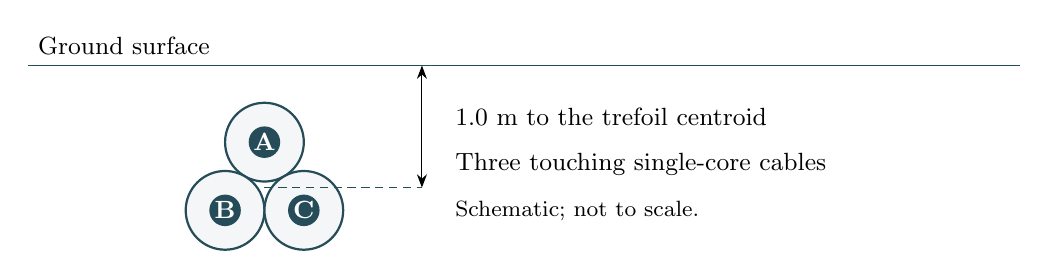
\begin{tikzpicture}[x=1cm,y=1cm,>=Stealth,font=\small]
\draw[accent,thin] (0,2.2)--(12.6,2.2);
\node[anchor=south west] at (0,2.22) {Ground surface};
\coordinate (O) at (3,0.65);
\foreach \x/\y/\phase in {3/1.227/A,2.5/0.361/B,3.5/0.361/C}{
 \draw[accent,thick,fill=accent!5] (\x,\y) circle (0.5);
 \fill[accent] (\x,\y) circle (0.20);
 \node[white,font=\small\bfseries] at (\x,\y) {\phase};
}
\draw[densely dashed,accent] (O)--(5.0,0.65);
\draw[<->] (5,0.65)--(5,2.2);
\node[anchor=west] at (5.3,1.55) {\(1.0~\mathrm{m}\) to the trefoil centroid};
\node[anchor=west] at (5.3,0.95) {Three touching single-core cables};
\node[anchor=west,font=\footnotesize] at (5.3,0.35) {Schematic; not to scale.};
\end{tikzpicture}
\end{center}
Using the nominal outside diameter, the cable centre-to-centre spacing is
\[
 S=D_{\mathrm{nom}}=45.5~\mathrm{mm}.
\]

\begin{table}[H]
\centering
\caption{Properties of the surrounding soil and burial environment.}
\label{tab:soil}
\begin{tabularx}{\linewidth}{@{}Y l Y@{}}
\toprule
Property & Value & Basis\\
\midrule
Burial depth & \(1.0~\mathrm{m}\) & NKT rating condition [1]\\
Undisturbed soil temperature & \(15~^\circ\mathrm{C}\) & NKT rating condition [1]\\
Thermal resistivity & \(1.2~\mathrm{K\,m/W}\) & NKT rating condition [1]\\
Thermal conductivity & \(0.833~\mathrm{W/(m\,K)}\) & Reciprocal of thermal resistivity\\
Relative permittivity & \(10\) & Appendix C baseline [A]\\
Relative permeability & \(1\) & Nonmagnetic approximation [A]\\
Electrical conductivity & \(0.01~\mathrm{S/m}\) & Appendix C baseline [A]\\
\bottomrule
\end{tabularx}
\end{table}
The thermal conductivity follows directly from the rated soil thermal resistivity:
\[
 \kappa_{\mathrm{soil}}=\frac{1}{\rho_{\mathrm{th,soil}}}
 =\frac{1}{1.2}\simeq 0.833~\mathrm{W\,m^{-1}\,K^{-1}}.
\]

\subhead{Justification}
\textbf{Thermal consistency.}
The soil temperature, thermal resistivity, depth and arrangement follow the
manufacturer's rating. Thus, \(0.833~\mathrm{W/(m\,K)}\) replaces the illustrative
\(1.0~\mathrm{W/(m\,K)}\) in Appendix C. Soil properties are initially uniform
and constant; moisture migration and drying are neglected.

\textbf{Electrical properties.}
Appendix C provides a reproducible reference soil, rather than a measured site.
With intact screens idealised as continuous and grounded, the surrounding soil
has little influence on the electric field inside the XLPE.
If exterior soil currents affect the results, the assumed electrical soil
properties require a sensitivity check.

\textbf{Depth convention.}
The datasheet does not define the reference point for the \(1.0~\mathrm{m}\)
burial depth. In the FE geometry, it is measured from the ground surface to the
centroid of the trefoil. This is an explicit modelling convention.
\end{document}

